\documentclass[10pt,twocolumn,a4paper]{article}

% Tata letak (rekonstruksi gaya konferensi IEEE, dua kolom, A4)
\usepackage[a4paper,top=19mm,bottom=25mm,left=16mm,right=16mm,columnsep=6mm]{geometry}
\usepackage[T1]{fontenc}
\usepackage[utf8]{inputenc}
\usepackage{mathptmx}
\usepackage{microtype}
\usepackage{amsmath}
\usepackage{booktabs}
\usepackage{enumitem}
\usepackage{titlesec}
\usepackage[font=footnotesize,labelsep=period]{caption}
\usepackage{cite}
\usepackage{balance}
\usepackage{graphicx}
\usepackage{array}
\usepackage{tikz}
\usetikzlibrary{arrows.meta}

\newcommand{\cost}{\mathit{Cost}}

% Kolom paragraf rata kiri untuk tabel dua kolom (dipakai pada Tabel I--IV).
\newcolumntype{P}[1]{>{\raggedright\arraybackslash}p{#1}}

\renewcommand{\figurename}{Gambar}
\renewcommand{\tablename}{Tabel}
\renewcommand{\thetable}{\Roman{table}}
\captionsetup[table]{textfont=sc,labelfont=sc,labelsep=newline,justification=centering,skip=3pt}
\captionsetup[figure]{skip=3pt}

\renewcommand{\thesection}{\Roman{section}}
\renewcommand{\thesubsection}{\Alph{subsection}}
\titleformat{\section}{\centering\normalfont\small\scshape}{\thesection.}{0.5em}{}
\titleformat{\subsection}{\normalfont\small\itshape}{\thesubsection.}{0.5em}{}
\titlespacing*{\section}{0pt}{1.4ex plus .3ex minus .2ex}{0.8ex plus .2ex}
\titlespacing*{\subsection}{0pt}{1.1ex plus .3ex minus .2ex}{0.5ex plus .2ex}

\setlength{\parindent}{1.2em}
\setlength{\parskip}{0pt}
\setlength{\textfloatsep}{8pt plus 2pt minus 2pt}
\setlength{\dbltextfloatsep}{8pt plus 2pt minus 2pt}
\setlength{\floatsep}{6pt plus 2pt minus 2pt}
\setlength{\intextsep}{6pt plus 2pt minus 2pt}
\setlength{\abovedisplayskip}{3pt plus 1pt minus 1pt}
\setlength{\belowdisplayskip}{3pt plus 1pt minus 1pt}
\setlist{nosep,leftmargin=*,itemsep=1pt}
\setlength{\tabcolsep}{3pt}
\renewcommand{\arraystretch}{1.05}
\hyphenpenalty=3000
\tolerance=1500
\emergencystretch=1.5em
\pagestyle{empty}

\begin{document}

\twocolumn[{%
\centering
{\fontsize{16}{18}\selectfont Implementasi dan Pengujian Numerik Sistem Pendukung Keputusan AHP--TOPSIS untuk Prioritisasi Penempatan CCTV di Permukiman Mahasiswa Jatinangor\par}
\vspace{10pt}
{\normalsize Marvel Evan T.\quad Kezia Tabhita Smith\quad Ibnaty Farah Rabbany\par}
{\normalsize Achmad Faruq M.\quad Gabriella Marie Keira Wibawa\par}
\vspace{4pt}
{\footnotesize Program Studi Teknik Informatika, Fakultas MIPA, Universitas Padjadjaran, Sumedang, Indonesia\par}
\vspace{10pt}
\begin{minipage}{0.86\textwidth}
\footnotesize
\textbf{\textit{Abstrak}}---Penempatan kamera pengawas (CCTV) di permukiman mahasiswa Jatinangor masih sporadis akibat keterbatasan anggaran, sehingga dibutuhkan mekanisme prioritisasi yang terukur. Kajian sebelumnya menghasilkan model konseptual DSS berbasis \textit{Analytic Hierarchy Process} (AHP) dan \textit{Technique for Order Preference by Similarity to Ideal Solution} (TOPSIS), namun belum diwujudkan sebagai perangkat lunak. Makalah ini melaporkan implementasi model tersebut menjadi aplikasi web satu-berkas yang dapat dijalankan luring, serta pengujian numeriknya. Model memakai lima alternatif segmen gang (A1--A5), delapan kriteria urgensi risiko (C1--C8) yang dipisahkan dari kelayakan teknis dan biaya (C9 dan RAB), pembobotan AHP lintas tiga kelompok pemangku kepentingan, dan perankingan TOPSIS dengan alokasi anggaran bertahap di bawah plafon Rp\,15 juta per tahun. Dataset disusun \textit{hybrid}: angka riil level desa/kecamatan dari sumber sekunder publik sebagai kalibrasi, sedangkan sel per-segmen merupakan estimasi terdokumentasi. Hasil pengujian: matriks AHP konsisten (CR $=0{,}0104<0{,}10$); bobot terbesar pada riwayat kerawanan C1 ($23{,}95\%$), diikuti defisiensi penerangan C3 dan mobilitas malam C2 (masing-masing $14{,}29\%$); peringkat TOPSIS A3 ($0{,}6445$) $>$ A1 ($0{,}5774$) $>$ A4 ($0{,}4995$) $>$ A2 ($0{,}4638$) $>$ A5 ($0{,}1820$); alokasi menghasilkan dua titik pada Fase~1 (Rp\,14,0 juta), dua pada Fase~2 (Rp\,13,0 juta), dan satu pada Fase~3. Analisis sensitivitas $\pm20\%$ (16 run) memperlihatkan peringkat puncak A3 dan A1 stabil pada seluruh skenario, dengan pembalikan peringkat hanya antara A4 dan A2 pada 2 dari 16 skenario. Aplikasi mereproduksi angka model secara persis dan menyediakan verifikasi perhitungan yang dapat diaudit.\\[4pt]
\textbf{\textit{Kata kunci}}---Decision Support System, AHP, TOPSIS, penempatan CCTV, implementasi perangkat lunak, Jatinangor.
\end{minipage}
\vspace{8pt}
}]

\section{Pendahuluan}

Kecamatan Jatinangor, Kabupaten Sumedang, merupakan kawasan pendidikan tinggi yang padat: lebih dari 98.000 jiwa pada 12 desa menurut BPS Kabupaten Sumedang 2024 \cite{bps}, sedangkan data E-Office Desa mencatat 91.469 jiwa \cite{eoffice}, dengan kantong permukiman mahasiswa di Desa Sayang, Cikeruh, Hegarmanah, Cipacing, dan Cileles. Pertumbuhan indekos di sepanjang gang sempit belum diimbangi kapasitas pengawasan: penerangan jalan umum (PJU) tidak merata dan penempatan CCTV bersifat reaktif. Kondisi ini menempatkan keselamatan warga, khususnya mahasiswa, sebagai persoalan \textit{Smart Living and Safety}.

Dari sudut kriminologi lingkungan, pengawasan ruang publik bertumpu pada \textit{Crime Prevention Through Environmental Design} (CPTED) \cite{crowe} dan \textit{Routine Activity Theory} \cite{cohen}: kehadiran pengawas yang cakap dan visibilitas lingkungan menurunkan peluang kejahatan. Kendala utamanya adalah anggaran publik, ketersediaan tiang, pasokan listrik, dan jaringan. Keputusan pemasangan yang sporadis berisiko menciptakan titik buta, investasi tidak efisien, dan pelanggaran privasi (UU PDP No.~27/2022). Karena itu diperlukan pendekatan kuantitatif yang transparan dan terukur.

Kajian \textit{scoping review} sebelumnya \cite{wang2025,gonzalez2024,feizizadeh2025,ahmed2022,choi2025,kanj2024,kabashkin2025,baddour2026,almassawa2024,shiddiqy2025,zheng2025,yuhang2025}, yang dipandu PRISMA-ScR \cite{tricco}, memetakan literatur DSS dan menghasilkan model konseptual: alternatif segmen gang, struktur kriteria keselamatan, pembobotan AHP multistakeholder, dan perankingan TOPSIS dengan alokasi anggaran bertahap. Namun model tersebut berhenti pada tahap konseptual dan baru diuji dengan perhitungan manual. Celah yang diisi makalah ini adalah mewujudkan model itu menjadi perangkat lunak yang dapat dijalankan dan menguji keterlaksanaan numeriknya secara terprogram dan dapat diaudit.

Kontribusi makalah ini: (1) implementasi model DSS AHP--TOPSIS menjadi aplikasi web satu-berkas (luring) yang mencakup matriks keputusan, matriks perbandingan berpasangan AHP, perhitungan bobot dan rasio konsistensi, perankingan TOPSIS, alokasi anggaran bertahap, dan analisis sensitivitas; (2) penyusunan dataset \textit{hybrid} berbasis sumber sekunder publik sebagai kalibrasi; (3) verifikasi bahwa aplikasi mereproduksi angka model secara persis sehingga dapat diaudit.

\section{Landasan Teori dan Karya Terkait}

\subsection{AHP}
\textit{Analytic Hierarchy Process} \cite{saaty} menurunkan bobot kriteria dari perbandingan berpasangan pada skala Saaty 1--9. Bobot diperoleh dari eigenvektor utama matriks perbandingan; kualitas penilaian diperiksa melalui \textit{Consistency Ratio} $CR=CI/RI$, dan matriks dinyatakan konsisten bila $CR<0{,}10$.

\subsection{TOPSIS}
TOPSIS \cite{hwang} memeringkat alternatif berdasarkan kedekatan terhadap solusi ideal: normalisasi vektor, pembobotan, penentuan solusi ideal positif ($A^{+}$) dan negatif ($A^{-}$), lalu koefisien kedekatan $CC_i = D_i^{-}/(D_i^{+}+D_i^{-})$.

\subsection{Karya Terkait}
Tinjauan literatur terdahulu mengelompokkan arsitektur DSS keselamatan perkotaan menjadi lima pola: GIS-MCDM dan evaluasi skenario spasial, optimasi \textit{coverage}, \textit{expert-driven}, simulasi-DSS operasional, dan \textit{policy-MCDA}; kombinasi AHP untuk pembobotan dan TOPSIS untuk perankingan merupakan pasangan yang paling langsung dapat diadopsi \cite{kanj2024} serta diperkuat bukti komparasi \cite{baddour2026}. Berbeda dari studi kota metropolitan berinfrastruktur sensor kontinu, aplikasi ini menargetkan permukiman padat dengan data diskrit lokal dan anggaran terbatas.

\section{Metode dan Perancangan Sistem}

\subsection{Alternatif dan Unit Keputusan}
Unit keputusan bukan tingkat desa, melainkan segmen gang yang menjadi kandidat satu titik CCTV. Lima segmen representatif dirumuskan (Tabel~\ref{tab:alt}) berdasarkan tipologi kerawanan dan karakteristik spasial.

\begin{table}[t]
\caption{Alternatif Segmen (A1--A5)}
\label{tab:alt}
\centering
\footnotesize
\begin{tabular}{@{}c P{0.30\columnwidth} c@{}}
\toprule
Kode & Segmen & Desa \\
\midrule
A1 & Gang Kos Sayang & Sayang \\
A2 & Ruas Jalan Cikeruh & Cikeruh \\
A3 & Persimpangan Hegarmanah & Hegarmanah \\
A4 & Gang Cipacing & Cipacing \\
A5 & Ruas Jalan Cileles & Cileles \\
\bottomrule
\end{tabular}
\end{table}

\subsection{Kriteria}
Sembilan kriteria dibagi dua domain fungsi (Tabel~\ref{tab:krit}). Kriteria C1--C8 adalah kriteria urgensi yang seluruhnya berorientasi \textit{benefit} terhadap urgensi (skor lebih tinggi = lebih mendesak) dan diproses langsung oleh TOPSIS. Kriteria C9 (kelayakan teknis) dan biaya (RAB) dipisahkan sebagai kendala alokasi. Implementasi menggunakan ambang kelayakan operasional $C9\ge3$ dan plafon anggaran. Model konseptual menetapkan C9 sebagai kendala kelayakan berskala 1--5 tanpa menyebut angka ambang, sehingga nilai $C9\ge3$ ditetapkan sebagai kebijakan implementasi yang terdokumentasi.

\begin{table}[t]
\caption{Matriks Kriteria C1--C9}
\label{tab:krit}
\centering
\footnotesize
\begin{tabular}{@{}c P{0.34\columnwidth} c c@{}}
\toprule
Kode & Kriteria & Satuan & Domain \\
\midrule
C1 & Riwayat kerawanan & insiden/km/th & Urgensi \\
C2 & Mobilitas malam & orang/jam & Urgensi \\
C3 & Defisiensi PJU & skor 1--5 & Urgensi \\
C4 & Efisiensi coverage & m$^2$/titik & Urgensi \\
C5 & Kepadatan kos & kamar/km & Urgensi \\
C6 & Derajat simpul & cabang & Urgensi \\
C7 & Gap CCTV eksisting & meter & Urgensi \\
C8 & POI rentan & unit & Urgensi \\
C9 & Kesiapan tiang/listrik & skor 1--5 & Kelayakan \\
\bottomrule
\end{tabular}
\end{table}

\subsection{Dataset Hybrid dan Sumber}
Data publik tidak menyediakan nilai per-gang untuk kedelapan kriteria, sehingga dataset disusun \textit{hybrid}. Angka riil dari sumber sekunder dipakai sebagai kalibrasi: populasi desa (Cipacing 15.096; Hegarmanah 9.712; Sayang 8.474; Cikeruh 7.848; Cileles 6.331) \cite{eoffice}; statistik kriminalitas Kecamatan Jatinangor yang naik dari 11 (2022) ke 155 kasus (2023) dengan Jatinangor menjadi salah satu dari tiga wilayah prioritas \cite{kabarsumedang} dan klaim penurunan pada 2024 \cite{harapanrakyat}; jumlah kamar sewa Desa Hegarmanah sebanyak 4.250 unit \cite{hegarmanah}; serta bukti defisiensi PJU di ruas Cileles--Narongtong \cite{kapol} dan keluhan penerangan di Jatinangor \cite{sumedangtandang}. Sel per-segmen yang tidak tersedia diberi label estimasi terdokumentasi. Matriks keputusan disajikan pada Tabel~\ref{tab:x}.

\begin{table*}[t]
\caption{Matriks Keputusan (Data Hybrid)}
\label{tab:x}
\centering
\footnotesize
\begin{tabular}{@{}l cccccccc c c@{}}
\toprule
Alternatif & C1 & C2 & C3 & C4 & C5 & C6 & C7 & C8 & C9 & Biaya (Rp Jt) \\
\midrule
A1 & 4,2 & 120 & 4 & 380 & 85 & 2 & 450 & 8 & 4 & 6,5 \\
A2 & 2,1 & 350 & 2 & 650 & 40 & 3 & 180 & 12 & 5 & 5,0 \\
A3 & 3,5 & 280 & 3 & 520 & 55 & 5 & 320 & 15 & 4 & 7,5 \\
A4 & 3,8 & 80 & 5 & 290 & 60 & 2 & 600 & 4 & 3 & 8,0 \\
A5 & 1,5 & 160 & 3 & 420 & 30 & 2 & 250 & 5 & 4 & 5,5 \\
\bottomrule
\end{tabular}
\end{table*}

\subsection{Pembobotan AHP}
Bobot diturunkan dari matriks perbandingan berpasangan konsensus $8\times8$ (Tabel~\ref{tab:ahp}). Agregasi lintas pemangku kepentingan memakai rata-rata geometrik (Persamaan~\ref{eq:geo}). Konsistensi diperiksa dengan CR (Persamaan~\ref{eq:cr}) dan $RI=1{,}41$ untuk $n=8$.

\begin{equation}
a_{jk}=\left(\prod_{p=1}^{P} a_{jk}^{(p)}\right)^{1/P}
\label{eq:geo}
\end{equation}

\begin{equation}
CI=\frac{\lambda_{\max}-n}{n-1},\qquad CR=\frac{CI}{RI}
\label{eq:cr}
\end{equation}

\begin{table*}[t]
\caption{Matriks Perbandingan Berpasangan AHP ($8\times8$)}
\label{tab:ahp}
\centering
\footnotesize
\begin{tabular}{@{}l cccccccc@{}}
\toprule
 & C1 & C2 & C3 & C4 & C5 & C6 & C7 & C8 \\
\midrule
C1 & 1,00 & 2,00 & 2,00 & 3,00 & 2,00 & 4,00 & 2,00 & 2,00 \\
C2 & 0,50 & 1,00 & 1,00 & 2,00 & 1,00 & 3,00 & 2,00 & 1,00 \\
C3 & 0,50 & 1,00 & 1,00 & 2,00 & 1,00 & 3,00 & 2,00 & 1,00 \\
C4 & 0,33 & 0,50 & 0,50 & 1,00 & 0,50 & 2,00 & 1,00 & 0,50 \\
C5 & 0,50 & 1,00 & 1,00 & 2,00 & 1,00 & 2,00 & 1,00 & 1,00 \\
C6 & 0,25 & 0,33 & 0,33 & 0,50 & 0,50 & 1,00 & 0,50 & 0,50 \\
C7 & 0,50 & 0,50 & 0,50 & 1,00 & 1,00 & 2,00 & 1,00 & 1,00 \\
C8 & 0,50 & 1,00 & 1,00 & 2,00 & 1,00 & 2,00 & 1,00 & 1,00 \\
\bottomrule
\end{tabular}
\end{table*}

\subsection{Perankingan TOPSIS dan Alokasi Anggaran}
Matriks keputusan urgensi $X=[x_{ij}]$ ($m=5$, $n=8$) diproses: normalisasi vektor Euclidean (Persamaan~\ref{eq:norm}), pembobotan (Persamaan~\ref{eq:w}), solusi ideal (Persamaan~\ref{eq:ideal}), jarak Euclidean (Persamaan~\ref{eq:dist}), dan koefisien kedekatan (Persamaan~\ref{eq:cc}). Alokasi bertahap mengelompokkan alternatif menurut $CC_i$ ke fase tahunan selama subtotal biaya tidak melampaui plafon $B_k$ (Persamaan~\ref{eq:budget}).

\begin{equation}
r_{ij}=\frac{x_{ij}}{\sqrt{\sum_{k=1}^{m}x_{kj}^{2}}}
\label{eq:norm}
\end{equation}

\begin{equation}
v_{ij}=w_j r_{ij},\qquad \sum_{j=1}^{n} w_j = 1
\label{eq:w}
\end{equation}

\begin{equation}
A^{+}=\{\max_i v_{ij}\},\qquad A^{-}=\{\min_i v_{ij}\}
\label{eq:ideal}
\end{equation}

\begin{equation}
D_i^{+}=\sqrt{\sum_{j=1}^{n}(v_{ij}-v_j^{+})^2},\quad D_i^{-}=\sqrt{\sum_{j=1}^{n}(v_{ij}-v_j^{-})^2}
\label{eq:dist}
\end{equation}

\begin{equation}
CC_i=\frac{D_i^{-}}{D_i^{+}+D_i^{-}},\qquad 0\le CC_i\le 1
\label{eq:cc}
\end{equation}

\begin{equation}
\sum_{i\in \mathrm{Fase}\ k} Cost_i \le B_k
\label{eq:budget}
\end{equation}

\subsection{Analisis Sensitivitas}
Setiap bobot kriteria diubah $\pm20\%$ secara \textit{One-At-A-Time} (OAT); bobot lain direnormalisasi proporsional; TOPSIS dihitung ulang untuk memeriksa ketahanan peringkat.

\section{Implementasi Sistem}

\subsection{Arsitektur Perangkat Lunak}
Aplikasi diwujudkan sebagai satu berkas HTML mandiri (\texttt{index.html}) berisi antarmuka, logika AHP--TOPSIS, dan dataset. Tidak ada server maupun dependensi eksternal, sehingga dapat dijalankan langsung di peramban (luring); seluruh perhitungan berjalan di sisi klien. Mesin dipisahkan dari data (\textit{data-driven}): jumlah segmen alternatif dimuat dari dataset, sehingga kasus lima segmen resmi dan skenario perluasan 12 desa (simulasi) dapat dijalankan tanpa mengubah kode. Arsitektur fungsionalnya mengikuti empat lapis model konseptual (Gambar~\ref{fig:arsitektur}): \textit{input}, \textit{preprocessing}, \textit{decision engine}, dan \textit{output}.

\subsection{Modul}
Aplikasi terdiri atas modul: (1) matriks keputusan C1--C8, C9, dan biaya (dapat diedit, memicu perhitungan ulang); (2) AHP dengan pengisian segitiga atas dan resiprokal otomatis, perhitungan bobot via iterasi pangkat, $\lambda_{\max}$, CI, dan CR; (3) TOPSIS; (4) alokasi fase anggaran; (5) peta prioritas skematik (SVG) yang memetakan peringkat secara spasial; (6) sensitivitas OAT 16 run; (7) ekspor hasil ke CSV.

\subsection{Antarmuka}
Gambar~\ref{fig:app} memperlihatkan antarmuka aplikasi: panel ringkasan menampilkan CR, alternatif terprioritas, dan plafon anggaran; tabel data dan matriks AHP dapat diedit; hasil peringkat TOPSIS dan alokasi fase ditampilkan berurutan.

\begin{figure}[t]
\centering
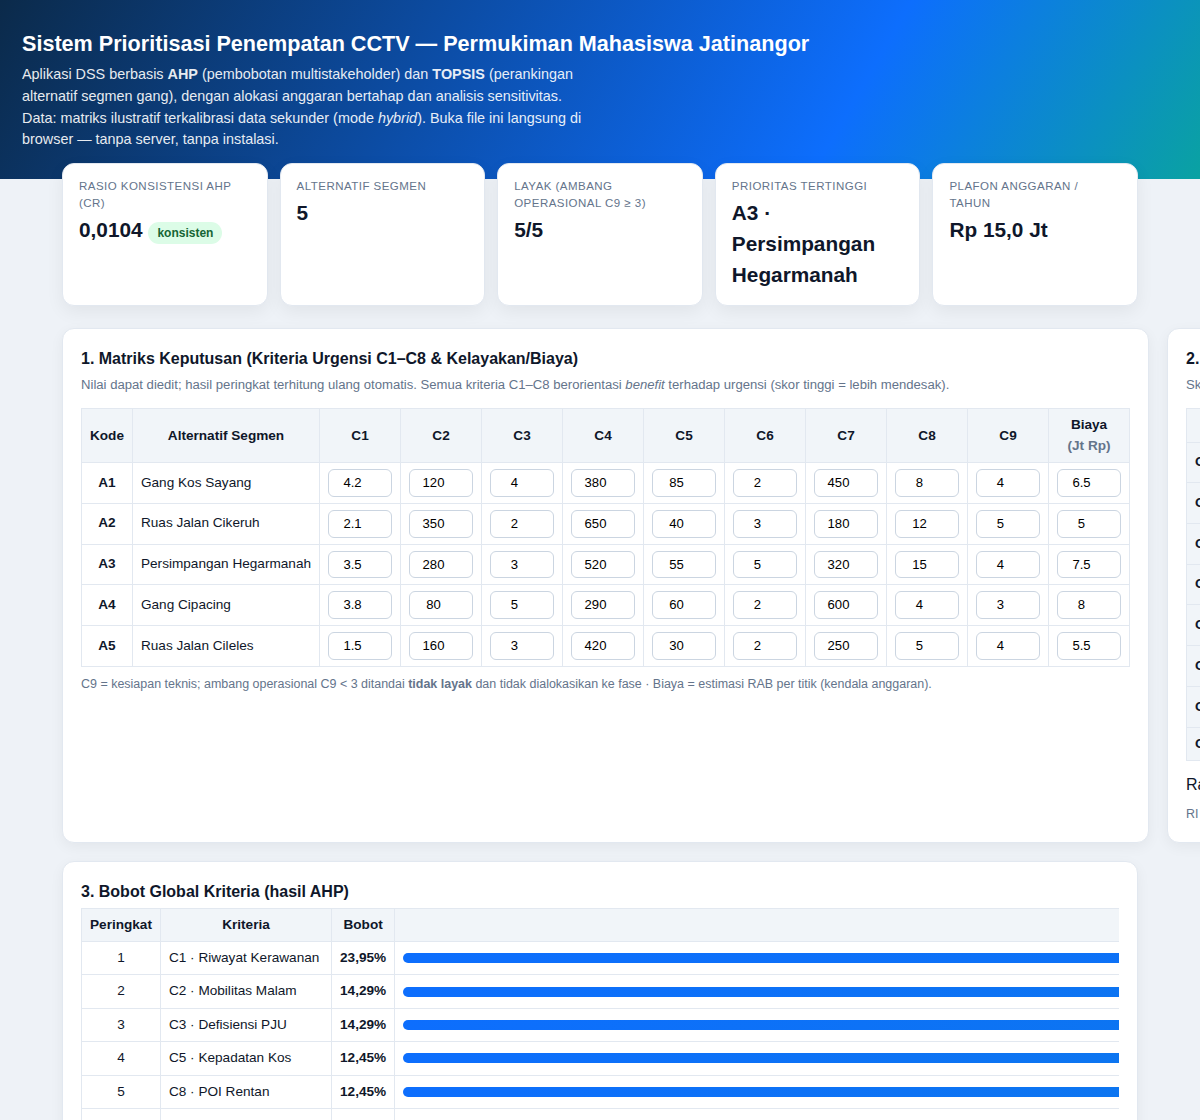
\includegraphics[width=\columnwidth]{img/aplikasi-screenshot.png}
\caption{Antarmuka aplikasi DSS prioritisasi CCTV Jatinangor.}
\label{fig:app}
\end{figure}

\begin{figure*}[!t]
\centering
% ============================================================================
% Arsitektur konseptual empat lapis DSS prioritisasi CCTV Jatinangor.
% SUMBER TUNGGAL gambar arsitektur untuk 04-paper dan 06-paper-hasil.
%
% Status: KANONIK (14 Nov 2026). Isi sudah diselaraskan dengan
% dss_revisi_markdown/dss_revisi.md: model AHP datar 8x8 (28 perbandingan),
% C1-C8 sebagai kriteria urgensi TOPSIS, C9 dan RAB sebagai kendala alokasi.
%
% Versi PNG lama (gambar-3-arsitektur.png / img/arsitektur.png) adalah
% artefak historis yang masih memuat "hierarki 3 kluster (10 pasang)" dan
% tidak boleh dipakai lagi.
%
% Prasyarat di preamble pemanggil: \usepackage{tikz}
%                                    \usetikzlibrary{arrows.meta}
%                                    \newcommand{\cost}{\mathit{Cost}}
% Pemakaian: dimuat di dalam lingkungan figure* (lebar penuh).
% ============================================================================
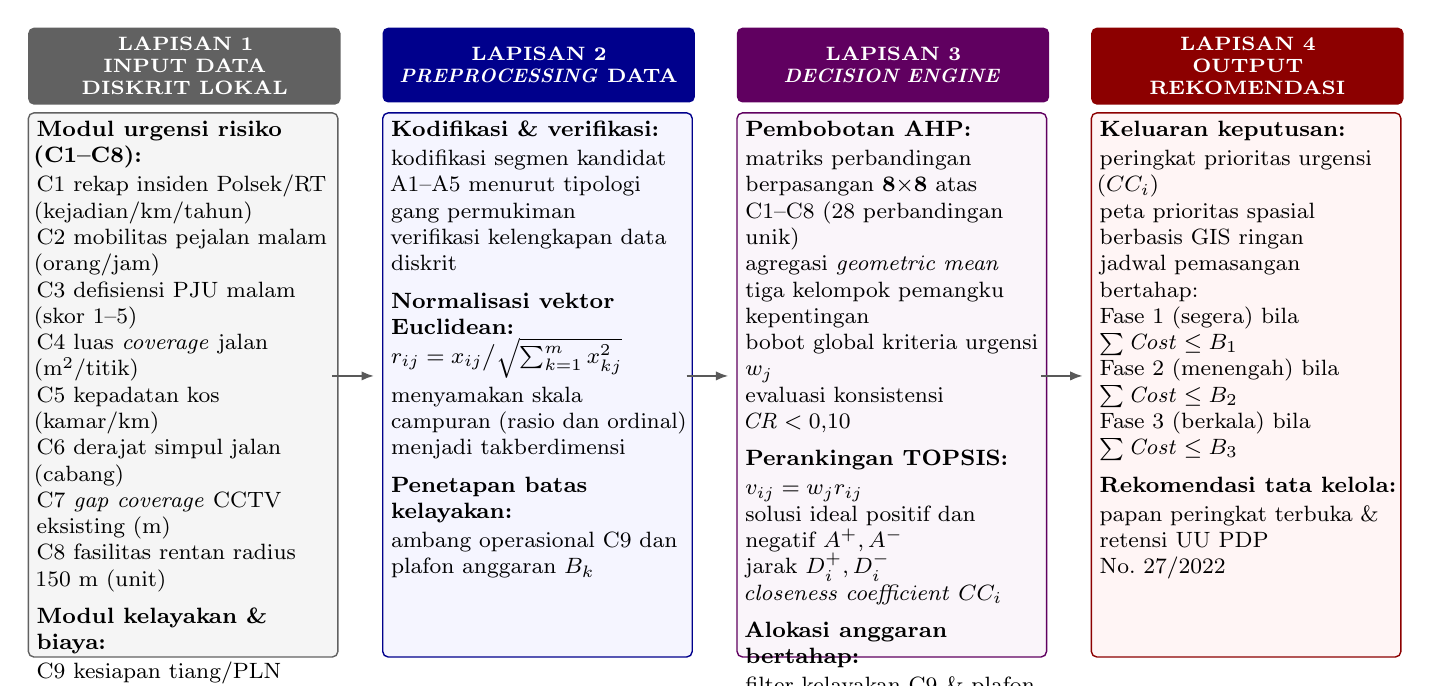
\begin{tikzpicture}[
    font=\footnotesize,
    layer/.style={
        draw, rounded corners=2pt, inner sep=3pt, line width=0.5pt,
        anchor=north west
    },
    head/.style={
        align=center, text width=3.72cm, text=white, font=\scriptsize\bfseries,
        inner sep=3.5pt, rounded corners=2pt, anchor=north west,
        minimum height=0.95cm
    },
    flow/.style={-{Latex[length=1.6mm]}, line width=0.8pt, draw=black!65}
]

% ---- judul lapisan -------------------------------------------------------
\node[head, fill=black!62]      (h1) at (0.00,0)  {LAPISAN 1\\INPUT DATA DISKRIT LOKAL};
\node[head, fill=blue!55!black] (h2) at (4.50,0)  {LAPISAN 2\\\textit{PREPROCESSING} DATA};
\node[head, fill=violet!75!black] (h3) at (9.00,0){LAPISAN 3\\\textit{DECISION ENGINE}};
\node[head, fill=red!55!black]  (h4) at (13.50,0) {LAPISAN 4\\OUTPUT REKOMENDASI};

% ---- isi lapisan (parbox Tinggi tetap -> kotak seragam, teks rata atas) ---
\node[layer, fill=black!4, draw=black!62] at (0.00,-1.08) {%
  \parbox[t][6.70cm][t]{3.72cm}{\raggedright%
    \textbf{Modul urgensi risiko (C1--C8):}\\[1pt]
    C1 rekap insiden Polsek/RT (kejadian/km/tahun)\\
    C2 mobilitas pejalan malam (orang/jam)\\
    C3 defisiensi PJU malam (skor 1--5)\\
    C4 luas \textit{coverage} jalan (m$^2$/titik)\\
    C5 kepadatan kos (kamar/km)\\
    C6 derajat simpul jalan (cabang)\\
    C7 \textit{gap coverage} CCTV eksisting (m)\\
    C8 fasilitas rentan radius 150 m (unit)\\[4pt]
    \textbf{Modul kelayakan \& biaya:}\\[1pt]
    C9 kesiapan tiang/PLN (skor 1--5)\\
    RAB pengadaan \& instalasi (juta Rp)%
  }%
};

\node[layer, fill=blue!4, draw=blue!55!black] at (4.50,-1.08) {%
  \parbox[t][6.70cm][t]{3.72cm}{\raggedright%
    \textbf{Kodifikasi \& verifikasi:}\\[1pt]
    kodifikasi segmen kandidat A1--A5 menurut tipologi gang permukiman\\
    verifikasi kelengkapan data diskrit\\[4pt]
    \textbf{Normalisasi vektor Euclidean:}\\[1pt]
    $r_{ij}=x_{ij}\big/\sqrt{\sum_{k=1}^{m}x_{kj}^{2}}$\\[2pt]
    menyamakan skala campuran (rasio dan ordinal) menjadi takberdimensi\\[4pt]
    \textbf{Penetapan batas kelayakan:}\\[1pt]
    ambang operasional C9 dan plafon anggaran $B_k$%
  }%
};

\node[layer, fill=violet!4, draw=violet!75!black] at (9.00,-1.08) {%
  \parbox[t][6.70cm][t]{3.72cm}{\raggedright%
    \textbf{Pembobotan AHP:}\\[1pt]
    matriks perbandingan berpasangan \textbf{8$\times$8} atas C1--C8 (28 perbandingan unik)\\
    agregasi \textit{geometric mean} tiga kelompok pemangku kepentingan\\
    bobot global kriteria urgensi $w_j$\\
    evaluasi konsistensi $\mathit{CR}<0{,}10$\\[4pt]
    \textbf{Perankingan TOPSIS:}\\[1pt]
    $v_{ij}=w_j r_{ij}$\\
    solusi ideal positif dan negatif $A^{+},A^{-}$\\
    jarak $D_i^{+},D_i^{-}$\\
    \textit{closeness coefficient} $CC_i$\\[4pt]
    \textbf{Alokasi anggaran bertahap:}\\[1pt]
    filter kelayakan C9 \& plafon biaya $B_k$%
  }%
};

\node[layer, fill=red!4, draw=red!55!black] at (13.50,-1.08) {%
  \parbox[t][6.70cm][t]{3.72cm}{\raggedright%
    \textbf{Keluaran keputusan:}\\[1pt]
    peringkat prioritas urgensi ($CC_i$)\\
    peta prioritas spasial berbasis GIS ringan\\
    jadwal pemasangan bertahap:\\
    Fase 1 (segera) bila $\sum \cost \le B_1$\\
    Fase 2 (menengah) bila $\sum \cost \le B_2$\\
    Fase 3 (berkala) bila $\sum \cost \le B_3$\\[4pt]
    \textbf{Rekomendasi tata kelola:}\\[1pt]
    papan peringkat terbuka \& retensi UU PDP No.~27/2022%
  }%
};

% ---- panah alur antar lapisan -------------------------------------------
\draw[flow] (3.87,-4.43) -- (4.40,-4.43);
\draw[flow] (8.37,-4.43) -- (8.90,-4.43);
\draw[flow] (12.87,-4.43) -- (13.40,-4.43);

\end{tikzpicture}

\caption{Arsitektur konseptual empat lapis DSS prioritisasi CCTV Jatinangor: lapisan input (data diskrit lokal C1--C9), lapisan \textit{preprocessing} (kodifikasi, verifikasi kelengkapan, normalisasi), lapisan \textit{decision engine} (AHP 8$\times$8 atas C1--C8, TOPSIS, alokasi anggaran), dan lapisan output (peringkat, peta prioritas, jadwal pemasangan bertahap). C9 dan RAB diperlakukan sebagai kendala alokasi, bukan kriteria TOPSIS.}
\label{fig:arsitektur}
\end{figure*}

\subsection{Verifikasi}
Algoritma aplikasi diuji terhadap hasil naskah konseptual melalui skrip pengujian berbasis Node.js. Pengujian memastikan reproduksibilitas bobot, CR, peringkat, alokasi fase, dan jumlah pembalikan peringkat. Seluruh nilai cocok pada toleransi $5\times10^{-4}$.

\section{Hasil dan Pembahasan}

\subsection{Bobot AHP dan Konsistensi}
Matriks pada Tabel~\ref{tab:ahp} menghasilkan $\lambda_{\max}=8{,}1031$, $CI=0{,}0147$, dan $CR=0{,}0104<0{,}10$, sehingga penilaian berpasangan konsisten. Vektor bobot global disajikan pada Tabel~\ref{tab:w}. Bobot terbesar pada riwayat kerawanan C1 ($23{,}95\%$), diikuti defisiensi penerangan C3 ($14{,}29\%$) dan mobilitas malam C2 ($14{,}29\%$). Urutan ini sejalan dengan tujuan keselamatan: kerawanan historis dan lingkungan gelap merupakan pemicu langsung risiko, sedangkan aspek spasial (C4, C6) berbobot lebih kecil karena bersifat pelengkap.

\begin{table}[t]
\caption{Bobot Global AHP}
\label{tab:w}
\centering
\footnotesize
\begin{tabular}{@{}c P{0.42\columnwidth} c@{}}
\toprule
Rank & Kriteria & Bobot \\
\midrule
1 & C1 Riwayat kerawanan & 23,95\% \\
2 & C2 Mobilitas malam & 14,29\% \\
3 & C3 Defisiensi PJU & 14,29\% \\
4 & C5 Kepadatan kos & 12,45\% \\
5 & C8 POI rentan & 12,45\% \\
6 & C7 Gap CCTV & 9,74\% \\
7 & C4 Efisiensi coverage & 7,70\% \\
8 & C6 Derajat simpul & 5,15\% \\
\bottomrule
\end{tabular}
\end{table}

\subsection{Perankingan TOPSIS}
Tabel~\ref{tab:topsis} menyajikan $D_i^{+}$, $D_i^{-}$, dan $CC_i$. Urutan urgensi: A3 $(0{,}6445) >$ A1 $(0{,}5774) >$ A4 $(0{,}4995) >$ A2 $(0{,}4638) >$ A5 $(0{,}1820)$. Persimpangan Hegarmanah (A3) menempati peringkat pertama karena mengombinasikan derajat simpul tinggi ($C6=5$), POI rentan banyak ($C8=15$), dan mobilitas malam tinggi; Gang Kos Sayang (A1) unggul pada kerawanan dan kepadatan kos. Ruas Cileles (A5) menempati peringkat terakhir karena hampir seluruh kriteria bernilai rendah.

\begin{table}[t]
\caption{Hasil Perankingan TOPSIS}
\label{tab:topsis}
\centering
\footnotesize
\begin{tabular}{@{}c P{0.40\columnwidth} c c c@{}}
\toprule
Rank & Alternatif & $D_i^{+}$ & $D_i^{-}$ & $CC_i$ \\
\midrule
1 & A3 Persimpangan Hegarmanah & 0,0646 & 0,1171 & 0,6445 \\
2 & A1 Gang Kos Sayang & 0,0865 & 0,1182 & 0,5774 \\
3 & A4 Gang Cipacing & 0,1094 & 0,1092 & 0,4995 \\
4 & A2 Ruas Jalan Cikeruh & 0,1119 & 0,0968 & 0,4638 \\
5 & A5 Ruas Jalan Cileles & 0,1447 & 0,0322 & 0,1820 \\
\bottomrule
\end{tabular}
\end{table}

\subsection{Visualisasi Prioritas Spasial}
Gambar~\ref{fig:peta} menampilkan peta prioritas skematik: tiap segmen digambar sebagai titik yang posisinya relatif terhadap koridor jalan utama Jatinangor; warna dan ukuran titik mengikuti nilai $CC_i$ (merah $=$ paling urgen), sedangkan label bawah menampilkan peringkat dan fase anggaran. Visualisasi ini membantu pemangku kepentingan membaca urutan prioritas secara spasial sebelum mengambil keputusan alokasi.

\begin{figure}[t]
\centering
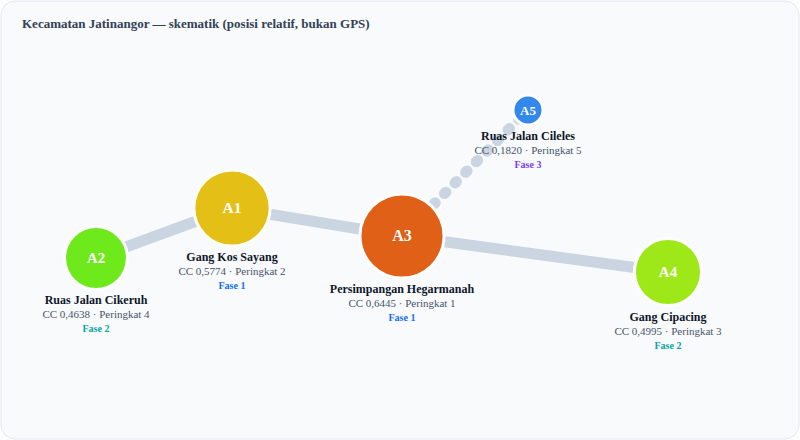
\includegraphics[width=\columnwidth]{img/peta-prioritas.png}
\caption{Peta prioritas skematik lima segmen CCTV Jatinangor.}
\label{fig:peta}
\end{figure}

\subsection{Alokasi Anggaran Bertahap}
Dengan plafon Rp\,15,0 juta per tahun, alternatif diurutkan menurut $CC_i$ lalu dikelompokkan (Tabel~\ref{tab:fase}). Setiap fase memenuhi plafon.

\begin{table}[t]
\caption{Alokasi Anggaran Bertahap}
\label{tab:fase}
\centering
\footnotesize
\begin{tabular}{@{}l l c c@{}}
\toprule
Fase & Alternatif & Biaya (Rp Jt) & Subtotal \\
\midrule
Fase 1 & A3, A1 & 7,5; 6,5 & 14,0 \\
Fase 2 & A4, A2 & 8,0; 5,0 & 13,0 \\
Fase 3 & A5 & 5,5 & 5,5 \\
\bottomrule
\end{tabular}
\end{table}

\subsection{Analisis Sensitivitas}
Tabel~\ref{tab:sens} menyajikan 16 run OAT ($\pm20\%$). Peringkat puncak A3 dan A1 stabil pada seluruh 16 skenario. Pembalikan peringkat hanya terjadi antara A4 dan A2 pada 2 dari 16 skenario, yaitu saat bobot C1 diturunkan $-20\%$ atau bobot C2 dinaikkan $+20\%$. Selisih $CC_i$ dasar keduanya relatif kecil ($0{,}4995$ vs $0{,}4638$), sehingga keduanya wajar ditempatkan pada satu paket Fase~2.

\begin{table*}[t]
\caption{Sensitivitas Bobot $\pm20\%$ (16 Run)}
\label{tab:sens}
\centering
\footnotesize
\begin{tabular}{@{}c c c c c c c l@{}}
\toprule
Kriteria & Variasi & A1 & A2 & A3 & A4 & A5 & Susunan \\
\midrule
C1 & $+20\%$ & 0,6157 & 0,4392 & 0,6570 & 0,5330 & 0,1660 & A3$>$A1$>$A4$>$A2$>$A5 \\
C1 & $-20\%$ & 0,5412 & 0,4849 & 0,6336 & 0,4699 & 0,1963 & A3$>$A1$>$A2$>$A4$>$A5 * \\
C2 & $+20\%$ & 0,5443 & 0,5010 & 0,6527 & 0,4695 & 0,1950 & A3$>$A1$>$A2$>$A4$>$A5 * \\
C2 & $-20\%$ & 0,6090 & 0,4270 & 0,6374 & 0,5276 & 0,1697 & A3$>$A1$>$A4$>$A2$>$A5 \\
C3 & $+20\%$ & 0,5805 & 0,4491 & 0,6280 & 0,5151 & 0,1914 & A3$>$A1$>$A4$>$A2$>$A5 \\
C3 & $-20\%$ & 0,5749 & 0,4760 & 0,6585 & 0,4867 & 0,1741 & A3$>$A1$>$A4$>$A2$>$A5 \\
C4 & $+20\%$ & 0,5745 & 0,4682 & 0,6445 & 0,4960 & 0,1847 & A3$>$A1$>$A4$>$A2$>$A5 \\
C4 & $-20\%$ & 0,5797 & 0,4602 & 0,6446 & 0,5024 & 0,1799 & A3$>$A1$>$A4$>$A2$>$A5 \\
C5 & $+20\%$ & 0,5898 & 0,4548 & 0,6354 & 0,5009 & 0,1769 & A3$>$A1$>$A4$>$A2$>$A5 \\
C5 & $-20\%$ & 0,5670 & 0,4710 & 0,6522 & 0,4984 & 0,1862 & A3$>$A1$>$A4$>$A2$>$A5 \\
C6 & $+20\%$ & 0,5735 & 0,4631 & 0,6466 & 0,4970 & 0,1812 & A3$>$A1$>$A4$>$A2$>$A5 \\
C6 & $-20\%$ & 0,5806 & 0,4643 & 0,6429 & 0,5016 & 0,1827 & A3$>$A1$>$A4$>$A2$>$A5 \\
C7 & $+20\%$ & 0,5790 & 0,4532 & 0,6327 & 0,5107 & 0,1815 & A3$>$A1$>$A4$>$A2$>$A5 \\
C7 & $-20\%$ & 0,5761 & 0,4725 & 0,6546 & 0,4903 & 0,1824 & A3$>$A1$>$A4$>$A2$>$A5 \\
C8 & $+20\%$ & 0,5667 & 0,4761 & 0,6605 & 0,4795 & 0,1774 & A3$>$A1$>$A4$>$A2$>$A5 \\
C8 & $-20\%$ & 0,5863 & 0,4535 & 0,6306 & 0,5170 & 0,1859 & A3$>$A1$>$A4$>$A2$>$A5 \\
\bottomrule
\end{tabular}
\end{table*}

\subsection{Verifikasi Implementasi}
Skrip pengujian mengekstrak blok \texttt{<script>} dari \texttt{index.html} dan menjalankannya di Node \texttt{vm} dengan DOM stub, sehingga yang diuji adalah kode aplikasi yang sebenarnya. Hasilnya, aplikasi mereproduksi angka naskah konseptual secara persis: $CR=0{,}0104$; bobot C1 $=23{,}95\%$; dan $CC_i$ A3 $=0{,}6445$, A1 $=0{,}5774$, A4 $=0{,}4995$, A2 $=0{,}4638$, A5 $=0{,}1820$. Hasil ini menegaskan bahwa alur komputasi model dapat dijalankan secara runtut dan direproduksi, sehingga kandidat penerapan di tingkat lokal menjadi lebih realistis.

\subsection{Keterbatasan}
Dataset bersifat \textit{hybrid}: angka per-segmen merupakan estimasi terdokumentasi, sehingga hasil belum merupakan validasi empiris dan perlu digantikan data survei lapangan (geometri gang, \textit{counting} mobilitas malam, survei PJU, pemetaan GPS CCTV, RAB). Bobot AHP merupakan penilaian konsensus ilustratif; bobot empiris harus diturunkan melalui kuesioner perbandingan berpasangan kepada pemangku kepentingan riil. Jumlah alternatif dibatasi lima segmen representatif; aplikasi menyediakan skenario perluasan 12 segmen (simulasi) untuk menunjukkan skalabilitas, tetapi perluasan ke data lapangan nyata belum diuji. Korelasi antarkriteria belum dimodelkan (peluang riset lanjutan dengan ANP).

\section{Kesimpulan}

Model DSS prioritisasi penempatan CCTV untuk permukiman mahasiswa Jatinangor telah diimplementasikan menjadi aplikasi web satu-berkas yang dapat dijalankan luring dan mereproduksi hasil numerik model secara persis. Pengujian menunjukkan matriks AHP konsisten ($CR=0{,}0104<0{,}10$) dengan bobot dominan pada riwayat kerawanan (C1, $23{,}95\%$); peringkat TOPSIS menempatkan Persimpangan Hegarmanah (A3) dan Gang Kos Sayang (A1) sebagai dua prioritas teratas; dan alokasi anggaran bertahap menghasilkan jadwal pemasangan yang memenuhi plafon Rp\,15 juta per tahun. Analisis sensitivitas $\pm20\%$ menunjukkan peringkat puncak stabil pada seluruh 16 skenario. Ke depan, model perlu diisi data survei lapangan dan bobot empiris pemangku kepentingan, diperluas ke lebih banyak segmen, dan ditingkatkan menjadi dasbor pemetaan spasial interaktif dengan koordinat GPS sebenarnya (saat ini tersedia peta prioritas skematik).

\balance
\begin{thebibliography}{99}
\footnotesize
\bibitem{bps} Badan Pusat Statistik Kabupaten Sumedang, \textit{Kecamatan Jatinangor Dalam Angka 2024}. Sumedang, Indonesia: BPS Kabupaten Sumedang, 2024.
\bibitem{crowe} T.\ D.\ Crowe, \textit{Crime Prevention Through Environmental Design}, 2nd ed. Boston, MA, USA: Butterworth-Heinemann, 2000.
\bibitem{cohen} L.\ E.\ Cohen and M.\ Felson, ``Social change and crime rate trends: A routine activity approach,'' \textit{Am. Sociol. Rev.}, vol.\ 44, no.\ 4, pp.\ 588--608, 1979.
\bibitem{saaty} T.\ L.\ Saaty, \textit{The Analytic Hierarchy Process: Planning, Priority Setting, Resource Allocation}. New York, NY, USA: McGraw-Hill, 1980.
\bibitem{hwang} C.-L.\ Hwang and K.\ Yoon, \textit{Multiple Attribute Decision Making: Methods and Applications}. Berlin, Germany: Springer-Verlag, 1981.
\bibitem{tricco} A.\ C.\ Tricco \textit{et al.}, ``PRISMA extension for scoping reviews (PRISMA-ScR): Checklist and explanation,'' \textit{Ann. Intern. Med.}, vol.\ 169, no.\ 7, pp.\ 467--473, Oct.\ 2018, doi: 10.7326/M18-0850.
\bibitem{wang2025} L.\ Wang, Y.\ Zhang, T.\ Feng, and X.\ Qi, ``Monitoring layout and optimisation method based on minimum weighted vertices of roads,'' \textit{Appl. Sci.}, vol.\ 15, no.\ 21, Art.\ no.\ 11622, 2025.
\bibitem{gonzalez2024} J.\ Gonz\'alez-Villa \textit{et al.}, ``Decision-support system for safety and security assessment and management in smart cities,'' \textit{Multimedia Tools Appl.}, vol.\ 83, no.\ 22, pp.\ 61971--61994, 2024.
\bibitem{feizizadeh2025} B.\ Feizizadeh and D.\ Omarzadeh, ``A GIS based spatiotemporal modelling approach for cycling risk mapping,'' \textit{Ann. GIS}, vol.\ 31, no.\ 2, pp.\ 333--351, 2025.
\bibitem{ahmed2022} V.\ Ahmed, S.\ Saboor, N.\ Ahmad, and M.\ Ghaly, ``A multi-attribute utility decision support tool for a smart campus: UAE as a case study,'' \textit{Front. Built Environ.}, vol.\ 8, Art.\ no.\ 1044646, 2022.
\bibitem{choi2025} J.\ Choi, J.\ Ok, and I.\ Yu, ``Smart city technologies for apartment complexes in South Korea: Expert prioritization and expected utility evaluation,'' \textit{J. Asian Archit. Build. Eng.}, early access, Dec.\ 2025.
\bibitem{kanj2024} H.\ Kanj, Y.\ Kotb, M.\ Alakkoumi, and S.\ Kanj, ``Dynamic decision making process for dangerous good transportation using a combination of TOPSIS and AHP methods with fuzzy sets,'' \textit{IEEE Access}, vol.\ 12, pp.\ 40450--40479, 2024.
\bibitem{kabashkin2025} I.\ Kabashkin \textit{et al.}, ``Synchronized multi-point UAV-based traffic monitoring for urban infrastructure decision support,'' \textit{Drones}, vol.\ 9, no.\ 5, Art.\ no.\ 370, 2025.
\bibitem{baddour2026} O.\ Baddour, A.\ Bhogayata, and T.\ Vora, ``Intelligent decision support for diplomatic quarter planning through multi-criteria analysis and urban intelligence,'' \textit{J. Intell. Decis. Mak. Inf. Sci.}, vol.\ 3, no.\ 3S, pp.\ 1612--1629, 2026.
\bibitem{almassawa2024} S.\ F.\ Almassawa, E.\ Rustiadi, A.\ Fauzi, and R.\ Sutriadi, ``Policy on the implementation of smart mobility in South Tangerang City, Indonesia using PROMETHEE,'' \textit{Plann. Malaysia}, vol.\ 22, no.\ 5, pp.\ 293--306, 2024.
\bibitem{shiddiqy2025} M.\ A.\ A.\ Shiddiqy \textit{et al.}, ``An integrated smart defense architecture for the Nusantara capital city of Indonesia,'' \textit{Int. J. Saf. Secur. Eng.}, vol.\ 15, no.\ 12, pp.\ 2561--2572, 2025.
\bibitem{zheng2025} X.\ Zheng, K.\ Wang, and M.\ Liu, ``A Bayesian Network and DEMATEL-ISM approach for smart community flood risk assessment,'' \textit{J. Cases Inf. Technol.}, vol.\ 27, no.\ 1, pp.\ 1--22, 2025.
\bibitem{yuhang2025} E.\ Yuhang \textit{et al.}, ``Sensor placement optimization for power grid condition monitoring based on a backup coverage model,'' \textit{Appl. Sci.}, vol.\ 15, no.\ 23, Art.\ no.\ 12570, 2025.
\bibitem{eoffice} Pemerintah Kabupaten Sumedang, ``Dashboard Desa Cantik / SAKIP Desa --- Kecamatan Jatinangor,'' E-Office Desa. [Online]. Available: https://e-officedesa.sumedangkab.go.id/dashboard\_simpatik/kecamatan/37
\bibitem{kabarsumedang} Kabar Sumedang, ``Tiga wilayah di Sumedang dengan tingkat kejahatan tinggi,'' 31 Des.\ 2023. [Online]. Available: https://kabarsumedang.pikiran-rakyat.com
\bibitem{harapanrakyat} Harapan Rakyat, ``Polres Sumedang klaim angka kriminalitas tahun 2024 turun signifikan,'' 31 Des.\ 2024. [Online]. Available: https://www.harapanrakyat.com/2024/12/polres-sumedang-klaim-angka-kriminalitas-tahun-2024-turun-signifikan/
\bibitem{kapol} KAPOL.ID, ``Jalan Narongtong-Cileles minim PJU,'' 12 Apr.\ 2021. [Online]. Available: https://kapol.id
\bibitem{sumedangtandang} Sumedang Tandang, ``Minimnya penerangan di Jatinangor dan dampaknya terhadap masyarakat,'' 18 Apr.\ 2023. [Online]. Available: https://sumedangtandang.com
\bibitem{hegarmanah} Pemerintah Desa Hegarmanah, ``Profil Desa Hegarmanah, Kecamatan Jatinangor,'' 2014. [Online]. Available: http://hegarmanah-jatinangor.blogspot.com/p/profil-desa.html
\end{thebibliography}

\end{document}
